\chapter{TIMER}
\section{Giới thiệu chung}
\subsection{Yêu cầu}
Sử dụng timer/counter trên vi điều khiển PIC 16F887 tạo thời gian trễ và tạo bộ đếm.
\subsection{Timer/Counter}
Timer được dùng để tạo ra khoảng thời gian trễ và nó cũng hoạt động như một bộ đếm (đếm số xung đi vào một chân cụ thể trên vi điều khiển).\\

Vi điều khiển PIC 16F887 có 3 bộ timer:
\begin{itemize}
\item \verb|Timer0|: $8$ bit, đếm được $255$, có chế độ định thời và bộ đếm.
\item \verb|Timer1|: $16$ bit, đếm được $65535$, có chế độ định thời và bộ đếm.
\item \verb|Timer2|: $8$ bit, có chức năng điều \verb|PWM| -- điều chế độ rộng xung.
\end{itemize}
\section{Các lệnh của Timer/Counter}
Gồm các lệnh sau:
\begin{itemize}
\item \verb|SETUP_TIMER_X(mode);| với \verb|X = 1| hoặc \verb|X = 2| (được định nghĩa trong \verb|device.h| (\verb|device| là tên chip)): khởi tạo \verb|TIMER|.
\item \verb|SET_TIMERx(value);| với \verb|x = 0| hoặc \verb|x = 1| hoặc \verb|x = 2|: thiết lặp giá trị bắt đầu cho \verb|TIMER|.
\item \verb|GET_TIMERx();| với \verb|x = 0| hoặc \verb|x = 1| hoặc \verb|x = 2|: đọc giá trị của \verb|TIMER/COUNTER|.
\end{itemize}

Xét cho từng bộ \verb|Timer|:
\begin{itemize}
\item \verb|TIMER0|: ta có các lệnh

\verb|SETUP_TIMER_0(mode);| \verb|SETUP_COUNTERS(rtcc_state, ps_state);| 

\verb|SET_TIMER0(value);| \verb|GET_TIMER0();|
\item \verb|TIMER1|: ta có các lệnh 

\verb|SETUP_TIMER_1(mode);| \verb|SET_TIMER1(value);| \verb|GET_TIMER1();|
\item \verb|TIMER2|: ta có các lệnh 

\verb|SETUP_TIMER_2(mode, period, postscale);| \verb|SET_TIMER2(value);| 

\verb|GET_TIMER2();|
\item[$\ast$] Các tham số (\verb|mode|, \verb|value|, \verb|rtcc_state|, \verb|ps_state|, \verb|period| và \verb|postscale|) của những hàm trên được định nghĩa trong thư mục \verb|DEVICES| ví dụ: \verb|16F887.h|, cách sử dụng những hàm này có thể xem trong phần \verb|Help| của phần mềm CCS.
\end{itemize}
\section{Bài tập}
\subsection{Bài tập 5.1}
\paragraph{Yêu cầu}Viết chương trình chớp tắt LED ở PORT E với thời gian delay $1s$ sửa dụng timer của PIC 16F887.
\paragraph{Hướng giải quyết}
\begin{itemize}
\item Đây là chương trình tạo thời gian trễ bằng cách sử dụng timer.
\item Chọn \verb|Timer0| $8$ bit để tạo thời gian trễ.
\item Tiến hành tính toán giá trị ban đầu cho thanh ghi \verb|TMR|: 
\begin{center}
\begin{tabular}{l|c|c|c|l|c}
\centering{Thông số} & Ký hiệu & Giá trị & Bộ chia & Giá trị &\verb|TMR0| \\ \hline
Tần số thạch anh & $F$ & $20MHz$ & $2$ & $2500$ & \\
Tần số lệnh & $\displaystyle F^\prime = \frac{F}{4}$ & $5MHz$ & $4$ & $1250$ &\\
Số xung trong $1s$ &  & $5 \times 10^6$ & $8$ & $625$ &\\
Số xung trong $1ms$ &  & $5 \times 10^3$ & $16$ & $312.5$ &\\
&  & & $32$ & $156.25$ & $256 - 156$\\
&  & & $64$ & $78.125$ &$= 100$\\
&  & & $128$ & $39.0625$ &\\
&  & & $256$ & $19.53125$ &\\
\end{tabular}
\end{center}
\begin{itemize}
\item Trong $1ms$ thực hiện $5 \times 10^3$ xung, mà \verb|Timer0| chỉ đếm được tới $255$. Nên chúng ta biến đổi số $5 \times 10^3$ qua các bộ chia trước.
\item Trong đó bộ chia trước $32$ là cho kết quả ít sai lệch so với các bộ chia khác. Chọn bộ chia $1:32$.
\item Thiết lập giá trị cho \verb|Timer0|: bộ \verb|Timer0| có $256$ giá trị, theo như cách chọn trên thì phải \verb|Timer0| phải đếm $156$ lần thì mới được $1ms$, nên cần phải cài đặt giá trị bắt đầu cho \verb|Timer0| là: $256 - 156 = 100$: \verb|SET_TIMER0(100);|
\end{itemize}
\item Sau khoảng thời gian đếm từ $100 \div 256$ thì \verb|Timer0| sẽ tràn, nên chúng ta sử dụng ngắt \verb|#INT_TIMER0| để xác định tràn trên \verb|Timer0|.
\item Để thời gian delay là $1s$, xác định số lần tràn như sau: $ count = 1 \times 1000$ lần.
\item Khai báo cho \verb|Timer0|: chọn xung kích nội và bộ chia trước $32$, giá trị ban đầu là $100$ rồi đếm lên, nên: \verb|SETUP_TIMER_0(RTCC_INTERNAL|$|$\verb|RTCC_DIV_32);| \verb|SET_TIMER0(100);|
\item Khai báo ngắt tràn trên \verb|Timer0|: \verb|ENABLE_INTERRUPTS(INT_TIMER0);| và thực hiện thiết kế chương trình ngắt như hướng dẫn ở \emph{mục \ref{Sec:int}} trong \emph{trang \pageref{Sec:int}}.
\item Chương trình ngắt: 
\begin{itemize}
\item Mỗi lần tràn \verb|Timer0| ta tăng biến \verb|count|.
\item So sánh biến \verb|count| với $1000$, nếu thỏa: \verb|count = 0;| và đảo trạng thái PORT E: \verb|PORTE =| $\sim$\verb|PORRTE|.
\end{itemize}
\item Thực hiện vòng lặp (dùng \verb|while|) để giữ cho vi điều kiển hoạt động.
\end{itemize}
\paragraph*{Sơ đồ mạch} Sơ đồ mạch giống sơ đồ mạch của \emph{bài tập 1.3} trong \emph{bài \ref{Les:1}}.
\subsection*{Chương trình 14}
\lstinputlisting[language=C]{BAI-5-1.C}
\subsection{Bài tập 5.2}
\paragraph{Yêu cầu}Viết chương trình đếm từ $0$ đến $9999$ sử dụng \verb|Timer| của \verb|PIC 16F887|, hiển thị trên \verb|LCD 16x02|.
\paragraph{Hướng giải quyết}
\begin{itemize}
\item Chúng ta sử dụng lại \emph{chương trình 14} để tạo thời gian trễ là \verb|sleep|, ví dụ trong chương trình khai báo \verb|int32 sleep = 500;| (tạo thời gian trễ $500ms$).
\item Chương trình ngắt: cứ sao một khoảng thời gian \verb|sleep| thì chúng ta tăng giá trị của biến \verb|dem| lên.
\item Chương trình chính: thêm vào vòng lặp \verb|while| công việc: hiện thị giá trị biến \verb|dem| lên \verb|LCD| (sử dụng hàm \verb|printf| kết hợp với hàm \verb|LCD_PutChar|). Thêm vào điều kiện so sánh, nếu vượt quá giới hạn, đặt lại biến \verb|dem = 0;|
\end{itemize}
\paragraph{Sơ đồ mạch}Giống sơ đồ mạch \emph{bài tập 2.3} trong \emph{bài \ref{Les:LCD}}.
\subsection*{Chương trình 15}
\lstinputlisting[language=C]{BAI-5-2.C}
\subsection{Bài tập 5.3}
\paragraph{Yêu càu}Viết chương trình đếm số lần nhấn phím sử dụng Timer của PIC 16F887, hiển thị trên LCD 16x02.
\paragraph{Hướng giải quyết}
\begin{itemize}
\item \verb|Timer 0| nhận được xung kích từ chân \verb|A4| của vi điều khiển (tùy thuộc vào cách ta cài đặt \verb|Timer 0|).
\item Cài đặt \verb|Timer 0|: \verb|SETUP_TIMER_0(RTCC_EXT_H_TO_L|$|$\verb|RTCC_DIV_1);| chọn bit cạnh xuống trên chân \verb|A4| và sử dụng bộ chia $1$ (do khi nhấn thì đếm và hiển thị lên \verb|LCD|, bộ chia $1$ là thích hợp nhất).
\item Cứ mỗi lần nhấn nút nhấn thì giá trị của \verb|Timer 0| tăng lên một giá trị. Sử dụng tính chất này để thực hiện đếm.
\item Thiết lập giá trị đầu cho \verb|Timer 0|: \verb|SET_TIMER0(0);| bắt đầu đếm từ 0.
\item Đọc giá trị của \verb|Timer 0|: \verb|value = GET_TIMER0();|. Chưa vội cho hiển thị giá trị \verb|value| lên LCD.
\item Do gặp phải vần đề sau: \verb|Timer 0| chỉ đếm được tới $255$, vượt quá $255$ thì chúng ta đếm sai, thực hiện kỹ thuật cộng dồn vào biến đếm: \verb|count = value + over*255|, với \verb|over| là số lần tràn (khi bắt đầu đếm thì \verb|over = 0;|)
\begin{itemize}
\item Chúng ta so sánh giá trị đọc được từ \verb|Timer 0| là biến \verb|value| với $255$ (giá trị tối đa của \verb|Timer 0|. Nếu \verb| value == 255| thì cho tăng biến \verb|over| lên.
\item Đồng thời cũng cần reset lại bộ đếm:\verb|SET_TIMER0(0);|
\end{itemize}
\item Phần còn lại, chúng ta chỉ việc cấu hình cho cho PORT A (chân \verb|INPUT|) và LCD rồi cho hiển thị giá trị của biến \verb|count| (đã thực hiện trong bài \ref{Les:LCD}).
\end{itemize}
\section*{Sơ đồ mạch}
\begin{figure}[!h]
\begin{center}
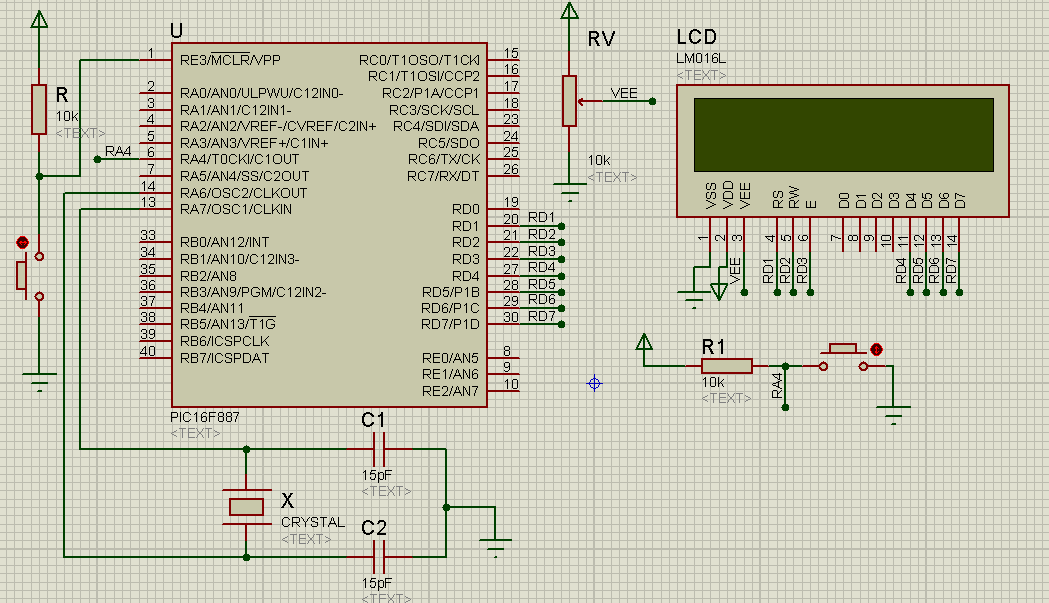
\includegraphics[scale=0.6]{bai-5/image/BAI-5-3}
\end{center}
\caption{Mạch đếm số lần nhấn nút sử dụng Timer hiển thị lên LCD}
\end{figure}
\newpage
\subsection*{Chương trình 16}
\lstinputlisting[language=C]{BAI-5-3.C}